\subsection{Specific Applications}
\label{subsec:03_applications}

In this section we take a closer look at applications that are linked to cybersecurity in a different way: Here the Blockchain is not per se used to mitigate direct cybersecurity threats but is used to make specific applications more robust, error-prone and less vulnerable.

\subsubsection{Assessment Criteria}
Below we want to introduce different scenarios of applications for the Blockchain technology and apart from a brief introduction of the challenges and problems of this specific field, answer the following questions:
\begin{itemize}
	\item What is the quality of this specific type of application regarding cybersecurity?
	\item How does the application make use of Blockchain Technology?
	\item Is the Blockchain really needed or could the problems be solved without it?
\end{itemize}
To answer these questions we are going to make use of the below schema presented by \citeauthor{Wust2017}, that helps to decide when to use a blockchain, what kind of blockchain to use, and when a use is not necessary.
\begin{figure}[ht!]
	\begin{center}
		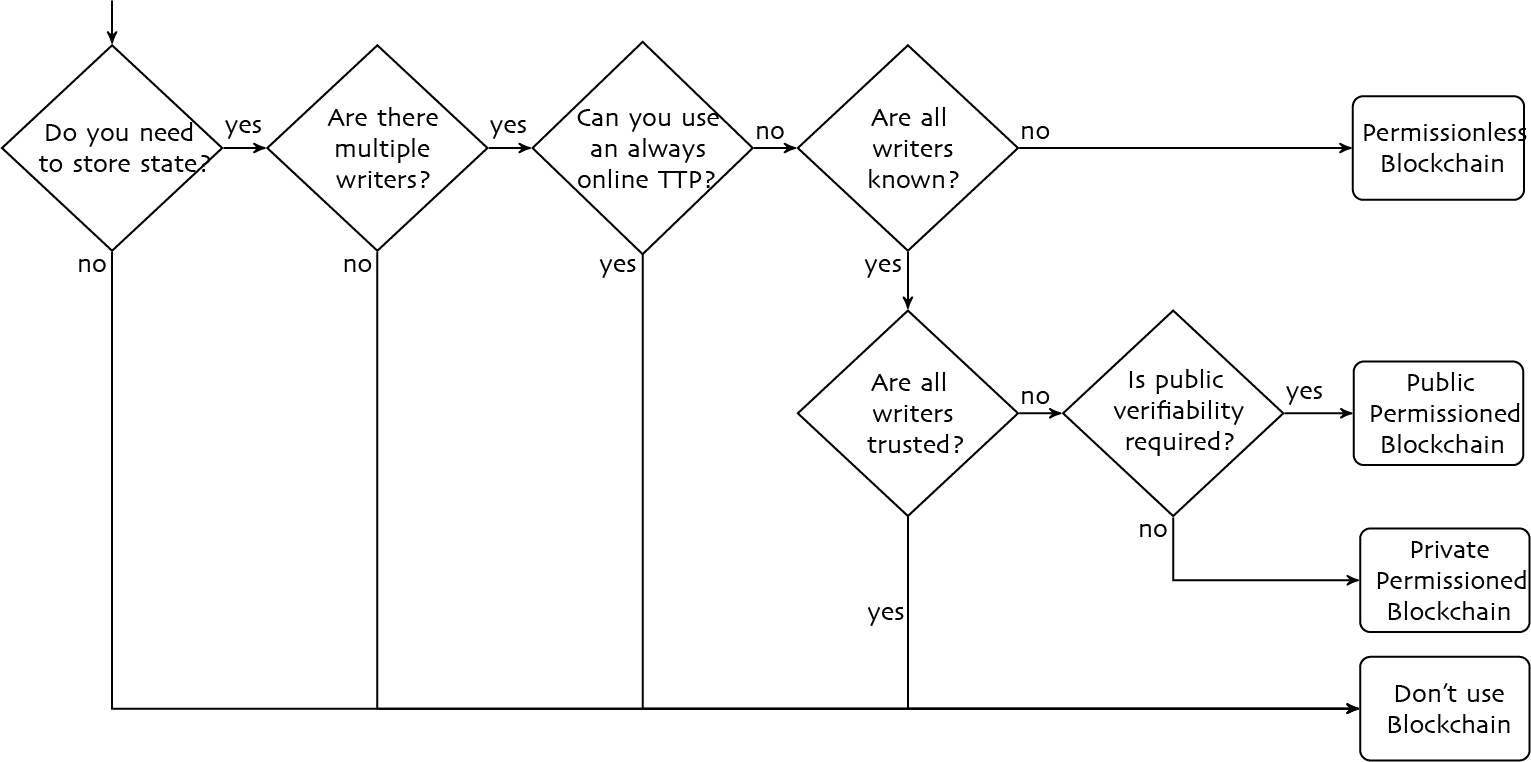
\includegraphics[scale=0.6]{Talk7/img/app/BCorNot}
	\end{center}
	\caption{Do you need a Blockchain?}
	\label{blockchain_or_not}
\end{figure}

\subsubsection{E-Voting}
The ability to vote is the very foundation of every successful democracy and must be accessible for all eligible citizens. Most common systems today are paper-based voting systems that do not scale well and rely on the procedural security of officials conducting their jobs.

Moreover, while various e-Voting systems exist, they all come with multiple security vulnerabilities, that lead to an enormous risk of election rigging and fraud.
The Blockchain, on the other hand, offers a transparent and incorruptible database that cannot have a single point of failure or be controlled by a single entity. It therefore immediately comes to mind, when thinking about a secure e-Voting system. Meanwhile new concerns arise, such as privacy and authentification issues.

To date, several e-Voring systems exist, that make use of the Blockchain technology. They all differ regarding the amount of integration and the role of the Blockchain. Different use cases, either in theory or in practice, have already been tested on smaller county elections or within private organizations. A quite exhaustive overview can be found in \citetitle{BenAyed2017} \cite{BenAyed2017}.

Most existing systems such as Votebook \cite{Kirby2016} or Vote Watchers \cite{BlockchainTechnologiesCorporation} still don't fully integrate the blockchain but instead use it as underlying database system in the form of a private permissioned blockchain. Those systems still rely on paper ballots. In such case, people have to authenticate by showing up in real life at a real voting booth. These two examples use of the Blockchain in the sense of a specific type of database, that is tamperproof and has the ability to create a history of all its entries. Additionally the results of each booth can be aggregated with all other stations to generate a final result in the end \cite{BenAyed2017}.
According to \citeauthor{Osgood2016}, these systems follow the only "doable" approach, as they dont deny the fact, that voters have to identify themselves somewhere.

Follow my Vote \cite{FollowMyVote} follows a fundamentally different approach: It really builds the application on top of the blockchain and uses its ability to act as a distributed ledger. Each voter installs a local "Voting Box" on his computer, equests ballots online and votes directily from within the application. The authentification process is done via the organization that holds the election by uploading official documents also from within the application. Nevertheless, according to \citeauthor{Osgood2016}, this idea is fundamentally flawed as authentication mechanisms are still an issue and the technique could scare off remote voters.

Within the three proposed systems, two fundamental questions seem to remain unanswered:
\begin{enumerate}
	\item \textbf{Authenticating users and the existence of a trusted third party}: The writers of the blockchain are either directly (via app) or indirectly (via real voting booth) the voters themselves. To authenticate them, an organization that has all the data about them is necessary. In most cases, this leaves only the government as an option. However, according to the diagram by \citeauthor{Wust2017} the use of Blockchain technology only makes sense if no trusted third party exists. This causes a dilemma: If the non-existing trust in the government is the justification for the use of the Blockchain, the question arises whether the government can be trusted regarding the authentication of the voters. Even though a systematic rigging is harder to achieve with this approach, the problem remains at hand.
	\item \textbf{The user as a single point of failure}: While the Blockchain does seem to be perfect for voting situations, its justification remains questionable. Especially, because it still leaves the most important point of failure unprotected: The user himself. Even the most tamper-proofed, blockchain-based voting system does not prevent hackers from a compromising and end-device.
\end{enumerate}

Many of the properties that are desired for e-Voting are provided by the Blockchain technology. But up to date, no system has yet been proposed that has been shown to be secure, verifiable and private at the same time. The question of authentification comes into play as an additional point of failure of the concept \cite{Osgood2016} .
Therefore, if an (online) trusted third party exists, the use of the blockchain is not necessary. If the government is trusted as far as the authentification of the voters goes, a public permissioned Blockchain can be a good fit. However, the security of the system then relies on the integrity of the validators, which leads us somehow where we started. If the government is not trusted at all, there exists no solution that overcomes that systematic flaw in a countries governance.

The Blockchain can be a solution if the question of authentification can be answered satisfactorily. Otherwise, a traditional paper-based voting system is as good as any voting system including Blockchain based systems or systems that base on a trusted third party.

\subsubsection{Autonomous Vehicles, Smart Cities \& IoT}
Smart vehicles are increasingly connected to infrastructure via the Internet, thus making them part of the IoT. This development brings apparent advantages, but also many challenges, especially in the area of cybersecurity. Malicious attacks on a vehicle endanger not only the vehicles data and passengers but also other road users. Also, while many common security and privacy methods exist to reduce the risk of an attack, they tend to be ineffective due to centralization, unscalability and unsecured communication architectures \cite{DorriSteger2017}.

The Blockchain offers solutions to many of the before mentioned problems. Therefore various approaches exist to connect self-driving vehicles with a blockchain-based architecture.

\citeauthor{DorriSteger2017} propose a smart vehicle ecosystem based on a blockchain architecture. It consists of clusters of nodes which are connected to the system via several nodes called Overlay Block Managers (OBMs). Each vehicle is connected to an overlay of various OBMs that form the nodes of the Blockchain based system. All Transactions are broadcast to and verified by the OBMs.
To ensure the user's privacy, each vehicle is equipped with internal vehicle storage to store sensitive data. It is the vehicle owner himself then, who defines which data is provided to third parties and which data is not.
To make specific Public Keys identifiable in the real world, a trusted third party is involved, and a centralized mechanism is used. This is needed in the case of service centers and software providers. The ecosystem makes remote software updates, vehicle insurance, smart charging, and vehicle sharing possible.

Also on a large scale, but slightly different is the hierarchical system proposed by \citeauthor{Sharma2017}. At the top exist two trusted third parties that register the vehicles (e.g., Department of Motor Vehicles) and that categorize the vehicles into minor nodes and ordinary nodes (Revocation Authority). Both parties exchange information with each other and the blockchain network. At the higher level, the blockchain overlay is constituted by controller nodes, that hold the information of the vehicle network and share it in a distributed manner with other controller nodes. The lower layer consists of minor nodes. These are selected vehicles that store data generated by sensors and applications. 
The hierarchy between the higher-order nodes and the lower-order nodes, allows to set different rights for different levels of the overlay: The system nodes e.g. are allowed to make specific data requests to the miner nodes, to gather information from sensors, while the miner nodes are only allowed to get general information from the higher-order nodes.

The paper by \citeauthor{Rowan2017} looks at the problem from a different angle: It focusses on the communication between two road members through side-channels such as visible light and acoustic signals. To solve the problem of the limited data throughput while trying to securely validate the other communication partner, centralized approaches were discarded due to the high number of existing manufacturers and standards. Instead, a blockchain based domain name system is proposed. This way of exchanging identity information was chosen as the most promising way of storing public keys due to its robustness and security regarding large scale attacks.

When two vehicles meet and try to authenticate each other, the communication  needs to be extremely fast and work in the absence of any internet connection or any centralized infrastructure. 
In this case, the Blockchain is used as a way to replace the need for a central authority when authenticating another vehicle. By creating a decentralized Name Service that binds the license plate value and identity together with a certificate, it is able to create a good base for a secure session between two vehicles.


The approach presented by \citeauthor{Sharma2017} is the only approach so far that thinks far beyond the incorporation of the blockchain into autonomous vehicles: It presents a framework for the controlled and secured interaction between all kinds of IoT devices. Cars as a particular case, are just one of them. The approach is very generally described, and the exact mechanisms that include the blockchain are not yet beyond an explanatory stage.
In the above ideas, the blockchain has different roles. And while the approach by \cite{Rowan2017} uses it as replacement for a domain name service, the approaches by \cite{DorriSteger2017} and \cite{Sharma2017} think further and propose actual ecosystems including other IoT devices in the use case of a smart city.
The thought of having multiple layers of nodes that, even though all incorporate the blockchain, have different rights to write and access it, seems very promising and suits well to the hierarchical structures that are necessary to organize a smart city network. In some way, it can be thought of a system of checks and balances where some nodes have more rights, but their actions can always be seen and verified from everywhere at any time.

Applying the flow-chart by \citeauthor{Wust2017}, we again identify the main issue again in the existence of a trusted third party. Whether it exists explicitly such as in the systems of \cite{Sharma2017} or implicitly such as in the case of \cite{Rowan2017} or \cite{DorriSteger2017}, in all three scenarios we have a third party that comes into play. 
Having a trusted third party available can only lead to two different outcomes according to \citeauthor{Wust2017}: Either, the use of the blockchain is not necessary or a private permissioned blockchain should be chosen \cite{Wust2017} and the blockchain gets reduced to a decentral database system.

By looking at the problems that an IoT network for autonomous vehicles faces, we can not identify a single problem that would make the use of the blockchain absolutely necessary. Forcing the blockchain onto such problems always leads to the same result: A private permissioned blockchain that is stripped off its real (decentral) powers in order to be controllable and easy to use. Therefore it is nothing else than another form of a database, that could be replaced with any other database architecture.

\subsubsection{Personal Data Protection and Sharing in the medical sector}
No field is more torn between data sharing and data protection like the medical sector. One one hand, sharing private data is necessary to ensure safe medication and even save lives; on the other hand, the data is extremely sensitive and can inflict big problems on individuals if made public.

In the health-care sector three traditional models exist to deal with the facility of interoperability of medical data \cite{Kshetri2017}: The push model, where medical information is sent from one provider to another, the pull model, where one provider asks another provider for information and the view model, where one provider looks at another providers record.
A major drawback to all of these models is that the data is not audited or tracked in a standardized way. For example, if a patient is transferred to a different hospital, the new hospital may not be able to access data that was not "pushed." This lack of audit trail means that there is no guarantee of data integrity from the point where data is generated to the point where it is used.
It is argued by \citeauthor{Kshetri2017} that the blockchain offers a fourth model, which makes it possible to share medical records securely across providers during the lifetime of a patient without having the need to include a trusted third party into the process. It leaves the data owner in full control about what is shared and leaves a verifiable audit trail of the data behind. \cite{Kshetri2017}

As an additional and particularly compelling aspect, the combination of IoT and the Blockchain in the healthcare sector needs to be mentioned. With the use of smart contracts, IoT devices carry out autonomous transactions on the Blockchain, while guaranteeing access control and data validity at the same time. Based on these thoughts various products and concepts have been created to make use of the Blockchain.

The MedRec system by \citeauthor{Azaria2016} is a blockchain-based, sophisticated network to share and protect clinical data. Via smart contracts on an Ethereum blockchain it logs patient-provider relationships that associate a medical record with viewing permissions and data retrieval instructions for the execution on external databases.
The systems nodes consist of providers, that require a full server and database infrastructure, and patients, that can use any mobile device or web-interface and use only a local database with their own data.
Providers can add new records associated with a particular patient and patients can authorize the sharing of records between providers. The involved parties are notified by automated notifications when changes occur or new data is added. To avoid unintended or abusive use of data, different policies are put in place by the owner and carried out by smart contracts
To create incentives to run a blockchain node, MedRec offers block rewards and anonymized patient data.

\citeauthor{Cao2019} focus on a different aspect and point out, that existing schemes cannot ensure the correctness and integrity of outsourced medical records. Especially not in the case, when authorized doctors collaborate with the cloud to modify records which are generated by the doctors themselves. \cite{Cao2019}

To address these problems, \citeauthor{Cao2019} propose a secure cloud-based system that runs without introducing any trusted third party.
When using this system, each patient makes an appointment with the hospital and obtains a treatment key for diagnosis. With the treatment key, a secure channel between patient and hospital and the doctors is established. 
The patient generates warrants to delegate to doctors, that indicate the identities of the treating doctors for specific treatment time and the needed auxiliary medical information.\cite{Cao2019}
During the treatment time, doctors generate medical records for the patient: In the multi-doctor use-case, medical records are successively generated by all treating doctors based on the record by the previous doctor. In such a case, a doctor is not only responsible for his own data, but also for the records his predecessors have generated. \cite{Cao2019}
The security of this system relies on the security of the Ethereum blockchain and the secure session established based on the treatment key. It is therefore protected against medical record modification attacks, impersonation attacks and a change of timeline whether by a hacker or an insider like a doctor.

While the approaches by \cite{Cao2019} and \cite{Azaria2016} both offer a different level of extensiveness, they both make good use of the blockchains ability to genereate an audit trail and run user-configurable smart contracts autonomously. 
The use of the blockchain is challenged again by the question "Are all writers trusted?"\cite{Wust2017}. It shows that the real problem lies int the transitioning part of the whole process: The moment when the real world gets projected by a human being onto the digital world, imposes the vulnerability.
If we do not trust the doctors to create rightful medical records, why do we consult them? Moreover, if we do trust them, why do we need a mechanism that prevents the doctors from forging medical records?

Disregarding of this fundamental problem, both systems provide proper security mechanisms against misuse of patient data and the falsification of patient data. The question whether such a system must be run on the blockchain can therefore not be answered finally. The Blockchain is used to make the system more secure. But the blockchain cannot take over the responsibility for human or institutional malevolence.

The whole field of IoT devices also includes the field of Wireless Body Area Networks (WBANs). In a WBAN a patient is equipped with one or multiple wearables or implanted medical devices, that take real-time measurements of vital indicators, such as heart rate or glucose levels. All devices report to one master device that collects and aggregates the data and offers a user-friendly interface.
The hereby existing security concerns are at hand: Live patient data is a lucrative target for hackers and poses not only a threat to the patient's health itself, but also to the privacy of its data.

To address these concerns, \citeauthor{Baccarini2018} propose integrating WBAN systems with smart contracts on a consortium-managed blockchain in order to provide a distributed data processing service, that creates an immutable log of the transactions between WBAN devices and the health care providers. \cite{Baccarini2018} This system allows for automatic notifications of health events to medical professionals in real time and in a secure manner.
In the presented system, the patients health monitor devices gather the raw data. The data of all devices gets collected and aggregated on a smartphone or a tablet and is then, together with customized threshold variables, sent to a specific smart contract on the blockchain. The smart contract evaluates the data and issues alerts to both patient and healthcare provider, as well as automated treatment instructions to the actuator nodes, if necessary.
No medical information is stored on the blockchain or in the smart contract. Instead, only the success (or failure) of the transactions gets stored. The data itself is forwarded to a designated storage database.
To authenticate the data later and to prevent and detect alterations, whether on purpose or accident, the blockchain transactions can be linked to the storage base where the patient's medical history lies.
The systems nodes consist of healthcare companies, which allows only designated members to read the blocks, execute smart contracts or verify new blocks.

Compared with traditional systems, a blockchain based system offers higher performance regarding the availability, the immutability, privacy as well as transparency of the data. Regarding confidentiality and speed, the proposed system performs worse or equal than traditional systems. \cite{Baccarini2018}
The most considerable challenge of the system is maintaining security at every individual node. Because the traffic of the master device of the WBAN is routed via the user's internet connection, the data is possibly transferred over an open channel.  Other challenges are key management on a large scale and the block verification times when the alert issued by the smart contract takes too long. \cite{Baccarini2018}

This system by \cite{Baccarini2018} fundamentally differs from the others in one aspect: The initially generated data is generated by an IoT device and is per se, digital. Therefore no translation step happens between the generation and the incorporation of the data.
Consequential, the system does not just use the blockchain as a replacement for any kind of database, but - especially in the combination with the smart contract - as a real entity that supports the interconnection of IoT devices with the service provider in a distributed, secure and tamper-proof manner. The fact that it does not use the blockchain to actually store data, but only to log the transitions emphasized this aspect.

In our opinion, the system by \citeauthor{Baccarini2018} is the only approach that has a real use for the design of the blockchain, without trying to alter its nature. The permissioned private blockchain used by the system is the right choice, to create maximum privacy, while at the same time distributing the data securely to the right place at the right time. \cite{Wust2017}

An uncovered topic in all the work on the blockchain in the medical sector is the "right to forget", as granted by the GDPR \cite{EuropeanCommission2017}. At least from a theoretical point of view, a traditional system allows the deletion of a record. Meanwhile, a blockchain based system does per design not make it possible to delete anything at all, as it is stored within the chain, in an unmodifiable way. In this regard, the papers of \cite{Cao2019} and \cite{Azaria2016}, that really store data on the blockchain itself, have to be treated as approaches that violate the GDPR.

\subsubsection{Concluding remarks}
The covered topics show a broad use of the blockchain in order to increase a systems security. Most of the time the blockchain is chosen as a way to store data in a tamperproof manner and to be able to verify the integrity of the data at all times.
Most approaches, however, try to create a suitable database system, that reduces the blockchain to a way of storing data in a distributed way. The result is always a private permissioned blockchain that has no real solution for the initial problem: The incorporation of the data itself into the blockchain. The human as the first actor and the problem that arises with this fact, namely that we cannot outsource trust to a machine, is neglected.

Promising, on the other hand, are use cases where such a human translation-factor does not exist per se. Use-cases that already have digital assets at hand, suit a blockchain scenario. Such approaches can exploit the advantages and properties of the blockchain technology at its fullest, without twisting it to fit a specific purpose.
